%
% related-work.tex
%
% Copyright (C) 2022 by SpaceLab.
%
% Camera Payload Preliminary Design Review
%
% This work is licensed under the Creative Commons Attribution-ShareAlike 4.0
% International License. To view a copy of this license,
% visit http://creativecommons.org/licenses/by-sa/4.0/.
%

%
% \brief Introduction slides.
%
% \author Gabriel Mariano Marcelino <gabriel.mm8@gmail.com>
% \author Vitória Beatriz Bianchin <vitoriabbianchin@gmail.com>
% \author Caique Sales de Miranda Gomes <kiqsmg@gmail.com>
%
% \version 0.1.0
%
% \date 2022/06/24
%


\begin{frame}{Comercial Cameras for CubeSats}

    A few commercial camera modules for CubeSats are available in the market:

    \begin{itemize}
        \item \href{https://gomspace.com/shop/payloads/earth-observation.aspx}{\textcolor{blue}{\underline{GomSpace NanoCam C1U}}}
        \vspace{0.4cm}
        \item \href{https://www.skyfoxlabs.com/product/27-digital-cubesat-camera}{\textcolor{blue}{\underline{SkyFox Labs piCAM}}}
        \vspace{0.4cm}
        \item \href{https://www.aac-clyde.space/what-we-do/space-products-components/payloads/im200}{\textcolor{blue}{\underline{AAC Hyperion IM200}}}
        \vspace{0.4cm}
        \item \href{https://redwirespace.com/products/spectracam}{\textcolor{blue}{\underline{RedWire SpectraCAM}}}
        \vspace{0.4cm}
        \item \href{https://dragonflyaerospace.com/products/gecko/}{\textcolor{blue}{\underline{Dragonfly Gecko Imager}}}
    \end{itemize}

\end{frame}

% #########################################################################
% #########################################################################

\begin{frame}{Comercial Cameras for CubeSats: \href{https://gomspace.com/shop/payloads/earth-observation.aspx}{\textcolor{cyan}{\underline{GomSpace NanoCam C1U}}}}

    \begin{columns}[t]
        \begin{column}[t]{0.6\textwidth}
            \begin{itemize}
                \item Res.: 3 MP (2048 $\times$ 1536 px)
                \item Sensor: Aptina MT9T031 (1/2'' CMOS)
                \item Lens: 8, 35 or 70 mm
                \item Processing:
                    \begin{itemize}
                        \item Processor: ARM
                        \item Memory: 512 MB RAM/2 GB flash
                    \end{itemize}
                \item Interfaces: CAN/I$^{2}$C
                \item Dimensions: 96 $\times$ 90 mm (PC104)
                \item Mass: 169 to 277 g
            \end{itemize}
        \end{column}
        \begin{column}[t]{0.4\textwidth}
            \vspace{0.7cm}
            \begin{figure}[!ht]
                \begin{center}
                    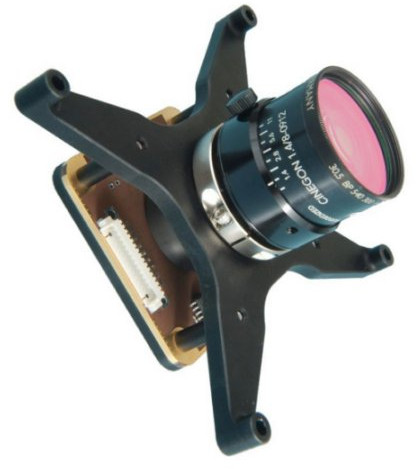
\includegraphics[width=4cm]{figures/nanocamc1u}
                \end{center}
            \end{figure}
        \end{column}
    \end{columns}

\end{frame}

% #########################################################################
% #########################################################################

\begin{frame}{Comercial Cameras for CubeSats: \href{https://www.skyfoxlabs.com/product/27-digital-cubesat-camera}{\textcolor{cyan}{\underline{SkyFox Labs piCAM}}}}

    \begin{columns}[t]
        \begin{column}[t]{0.65\textwidth}
            \begin{itemize}
                \item Res.: VGA (640 $\times$ 480 px)
                \item Sensor: Color RGB
                \item Lens: 76$^{\circ}$ (default), 116$^{\circ}$ or 170$^{\circ}$ (FoV)
                \item Interface: UART (115200 bps) 
                \item Consumption: 315 mW (typical)
                \item Dimensions: 48 $\times$ 33 $\times$ 40,5 mm
                \item Mass: 40 g
                \item Price: 4390 EUR (FM)
            \end{itemize}
        \end{column}
        \begin{column}[t]{0.35\textwidth}
            \begin{figure}[!ht]
                \begin{center}
                    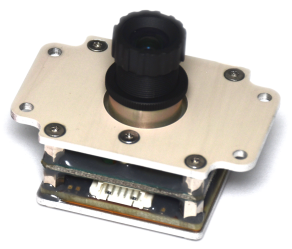
\includegraphics[width=3.5cm]{figures/picam-front}
                \end{center}
            \end{figure}
            \begin{figure}[!ht]
                \begin{center}
                    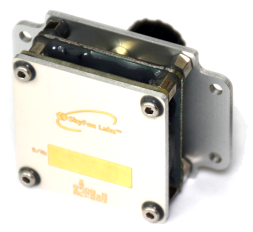
\includegraphics[width=3.5cm]{figures/picam-back}
                \end{center}
            \end{figure}
        \end{column}
    \end{columns}
    
\end{frame}

% #########################################################################
% #########################################################################

\begin{frame}{Comercial Cameras for CubeSats: \href{https://www.skyfoxlabs.com/product/27-digital-cubesat-camera}{\textcolor{cyan}{\underline{SkyFox Labs piCAM}}}}

    \begin{itemize}
        \item Examples (lens: 76$^{\circ}$, with IR-filter):
    \end{itemize}
    \begin{figure}[!ht]
        \begin{center}
            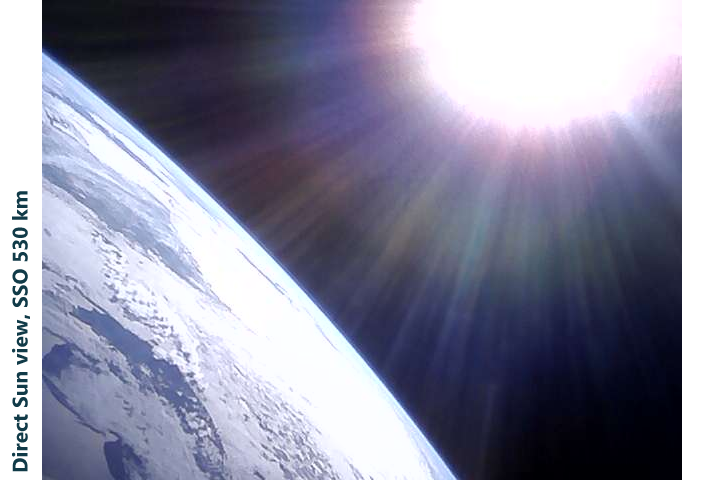
\includegraphics[width=9cm]{figures/picam-ex1}
        \end{center}
    \end{figure}

\end{frame}

\begin{frame}{Comercial Cameras for CubeSats: \href{https://www.skyfoxlabs.com/product/27-digital-cubesat-camera}{\textcolor{cyan}{\underline{SkyFox Labs piCAM}}}}

    \begin{figure}[!ht]
        \begin{center}
            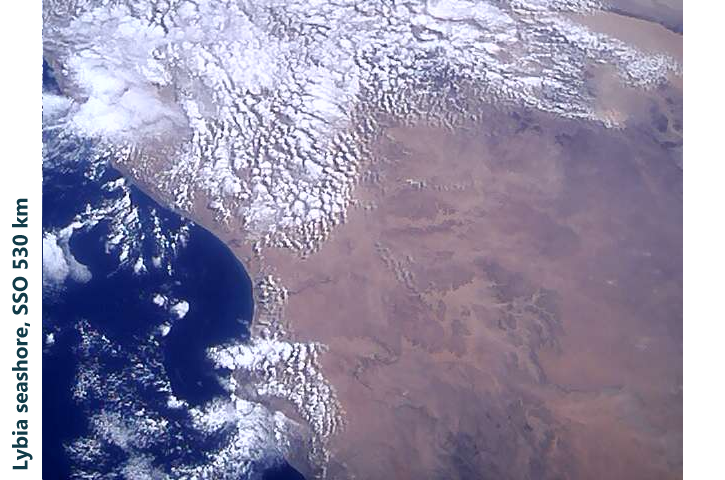
\includegraphics[width=10cm]{figures/picam-ex2}
        \end{center}
    \end{figure}

\end{frame}

\begin{frame}{Comercial Cameras for CubeSats: \href{https://www.skyfoxlabs.com/product/27-digital-cubesat-camera}{\textcolor{cyan}{\underline{SkyFox Labs piCAM}}}}

    \begin{figure}[!ht]
        \begin{center}
            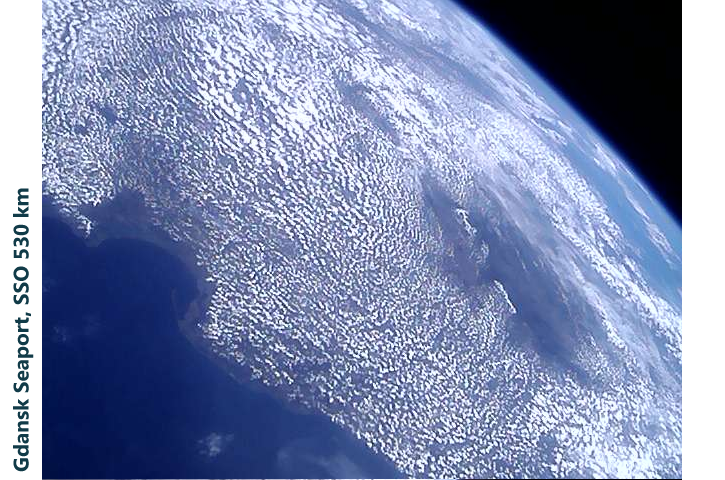
\includegraphics[width=10cm]{figures/picam-ex3}
        \end{center}
    \end{figure}

\end{frame}

% #########################################################################
% #########################################################################

\begin{frame}{Custom Projects: \href{http://www.madeinepal.com/2016/03/complete-guide-to-designing-camera.html}{\textcolor{cyan}{\underline{SNUSat}}}}

    \begin{columns}[t]
        \begin{column}[t]{0.6\textwidth}
            \begin{itemize}
                \item Res.: 2 MP (1600 $\times$ 1200 px)
                \vspace{0.2cm}
                \item Sensor: Micron MT9D111
                \vspace{0.2cm}
                \item Processing:
                    \begin{itemize}
                        \item Processor: STM32F4
                        \item Memory: 8 MB SDRAM/8 MB flash
                    \end{itemize}
                \vspace{0.2cm}
                \item Interface: I$^{2}$C
            \end{itemize}
        \end{column}
        \begin{column}[t]{0.5\textwidth}
            \begin{figure}[!ht]
                \begin{center}
                    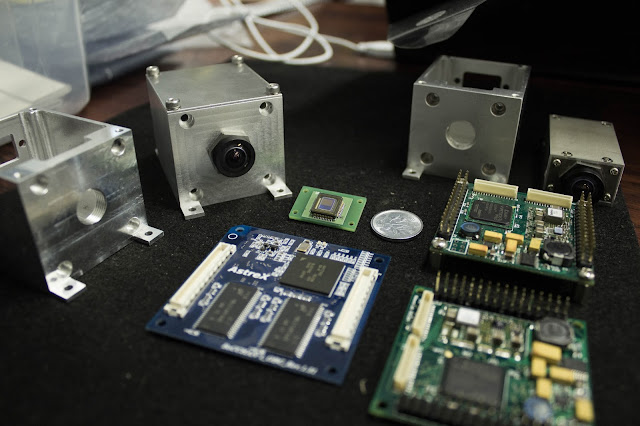
\includegraphics[width=5cm]{figures/snucam}
                \end{center}
            \end{figure}
            \begin{figure}[!ht]
                \begin{center}
                    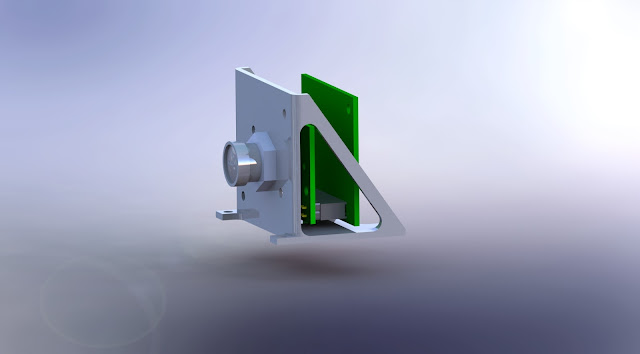
\includegraphics[width=5cm]{figures/snusat-cam-render}
                \end{center}
            \end{figure}
        \end{column}
    \end{columns}

\end{frame}

% #########################################################################
% #########################################################################

\begin{frame}{Custom Projects: \href{http://stf1.com/}{\textcolor{cyan}{\underline{STF-1}}}}

    \begin{columns}[t]
        \begin{column}[t]{0.6\textwidth}
            \begin{itemize}
                \item Launch: 2018
                \vspace{0.3cm}
                \item Image sensor module: ArduCam Mini 2MP Plus (same as planned for this project!!)
                \vspace{0.3cm}
                \item With active attitude control system (magnetorquers)
            \end{itemize}
        \end{column}
        \begin{column}[t]{0.4\textwidth}
            \begin{figure}[!ht]
                \begin{center}
                    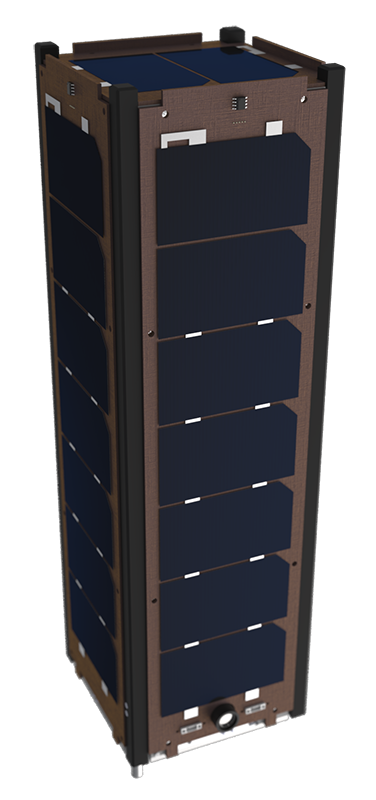
\includegraphics[width=3cm]{figures/stf1_closed_top.png}
                \end{center}
            \end{figure}
        \end{column}
    \end{columns}

\end{frame}

\begin{frame}{Custom Projects: \href{http://stf1.com/}{\textcolor{cyan}{\underline{STF-1}}}}

    \begin{columns}[t]
        \begin{column}[t]{0.4\textwidth}
            \begin{figure}[!ht]
                \begin{center}
                    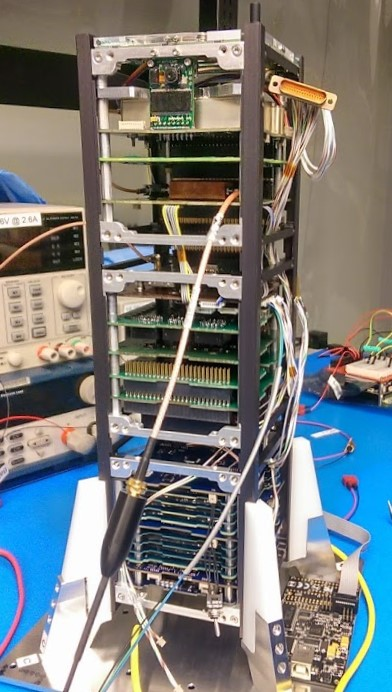
\includegraphics[width=3.5cm]{figures/stf1_integration-2.jpg}
                \end{center}
            \end{figure}
        \end{column}
        \begin{column}[t]{0.6\textwidth}
            \begin{figure}[!ht]
                \begin{center}
                    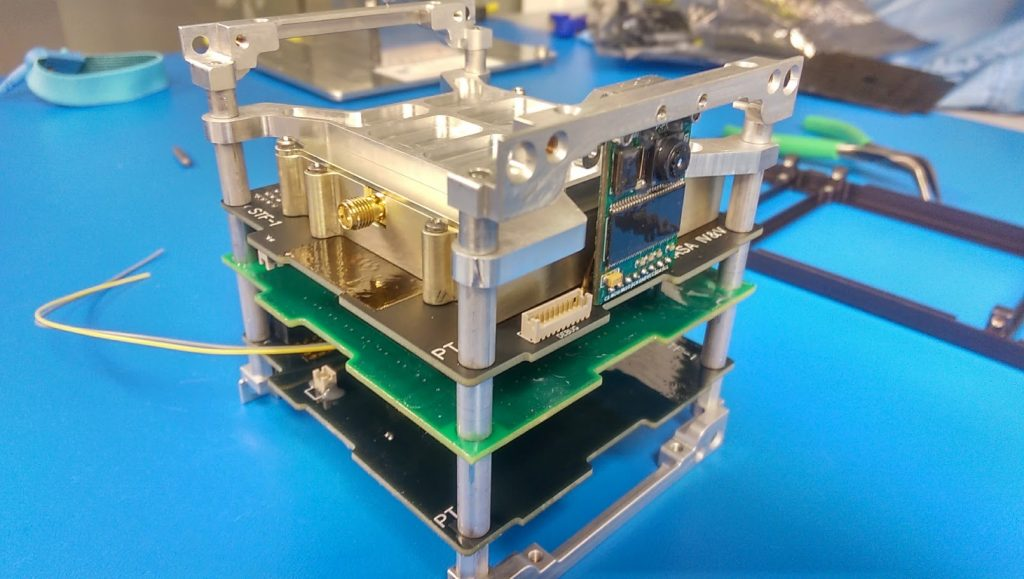
\includegraphics[width=5.5cm]{figures/stf1_stack_top-1024x579.jpg}
                \end{center}
            \end{figure}
            \begin{figure}[!ht]
                \begin{center}
                    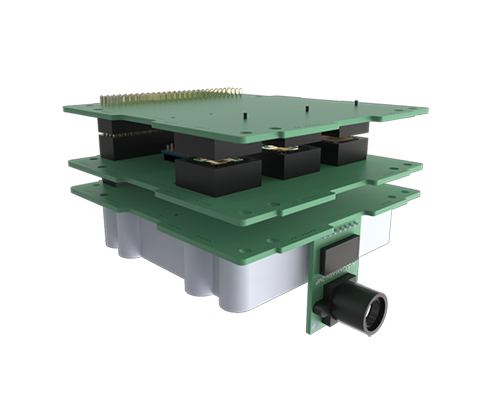
\includegraphics[width=4.5cm]{figures/stf1_bottom_cube.png}
                \end{center}
            \end{figure}
        \end{column}
    \end{columns}

\end{frame}

\begin{frame}{Custom Projects: \href{http://stf1.com/}{\textcolor{cyan}{\underline{STF-1}}}}

    In-flight pictures' examples:

    \begin{figure}[!ht]
        \begin{center}
            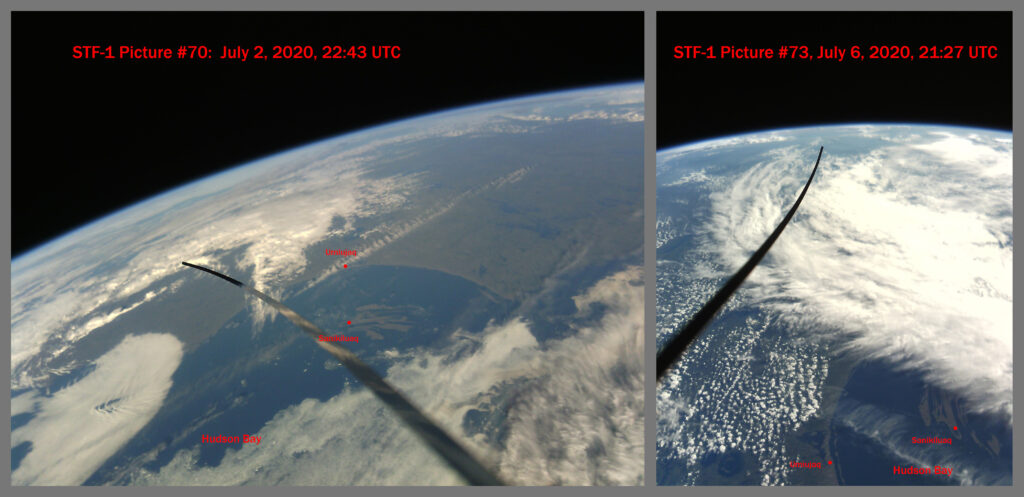
\includegraphics[width=10.5cm]{figures/stf-1-ex1.jpg}
        \end{center}
    \end{figure}

\end{frame}

\begin{frame}{Custom Projects: \href{http://stf1.com/}{\textcolor{cyan}{\underline{STF-1}}}}

    \begin{figure}[!ht]
        \begin{center}
            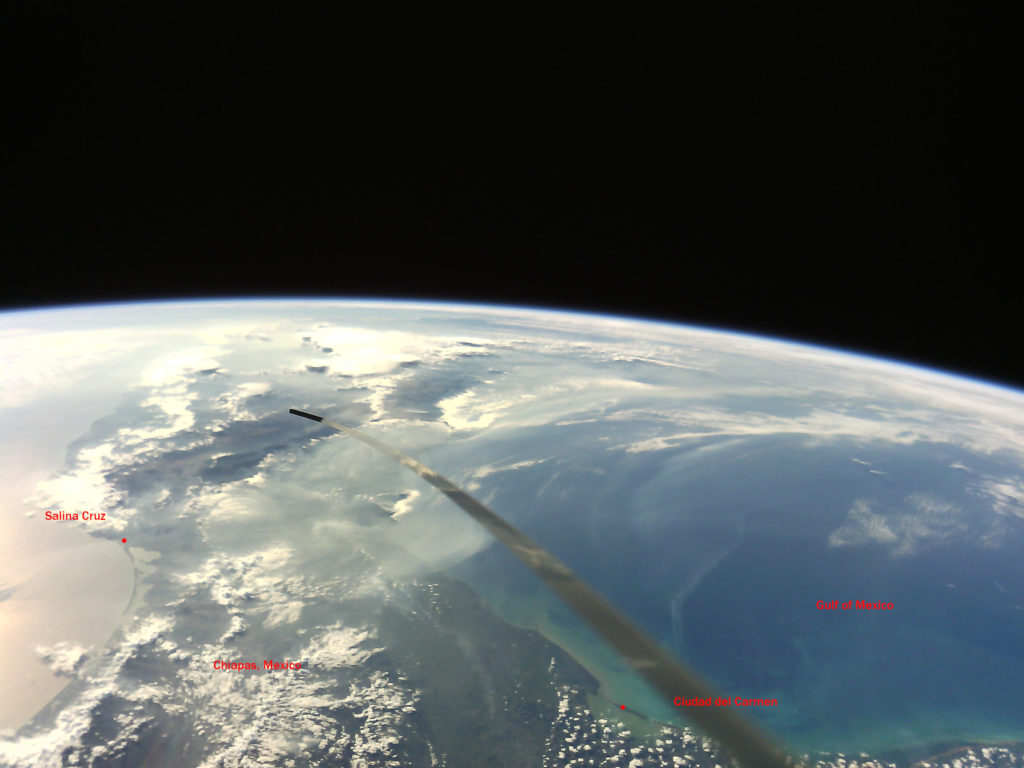
\includegraphics[width=9.5cm]{figures/stf-1-ex2.jpg}
        \end{center}
    \end{figure}

\end{frame}

\begin{frame}{Custom Projects: \href{http://stf1.com/}{\textcolor{cyan}{\underline{STF-1}}}}

    \begin{figure}[!ht]
        \begin{center}
            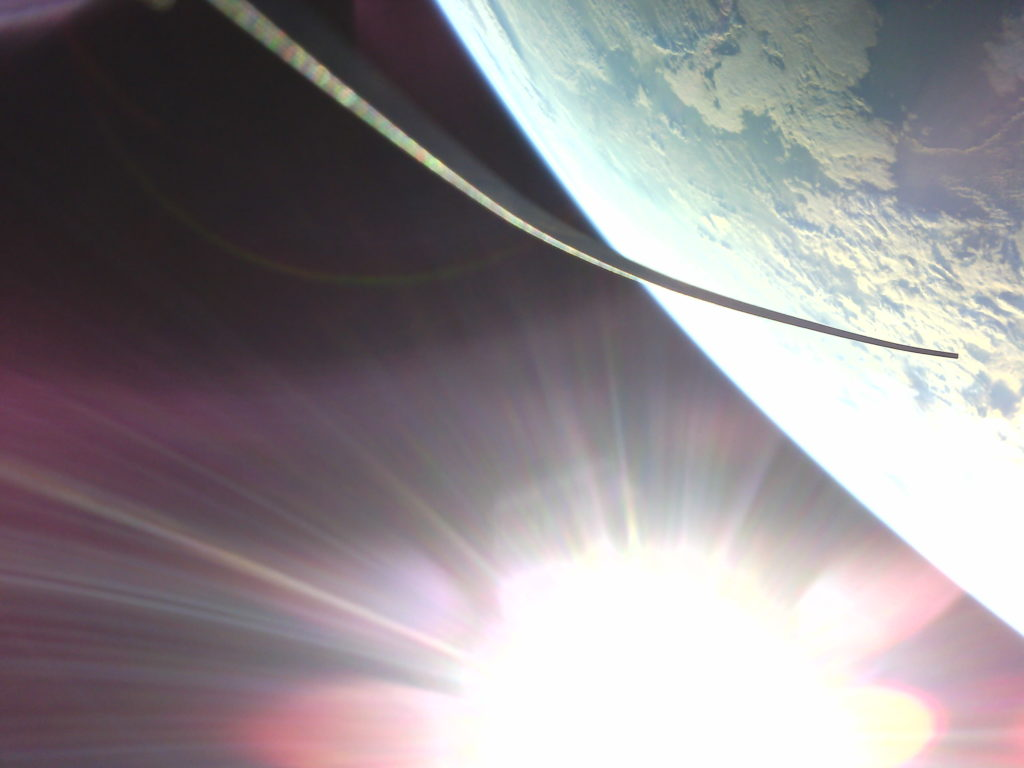
\includegraphics[width=9.5cm]{figures/stf-1-ex3.jpg}
        \end{center}
    \end{figure}

\end{frame}

\begin{frame}{Custom Projects: \href{http://stf1.com/}{\textcolor{cyan}{\underline{STF-1}}}}

    \begin{figure}[!ht]
        \begin{center}
            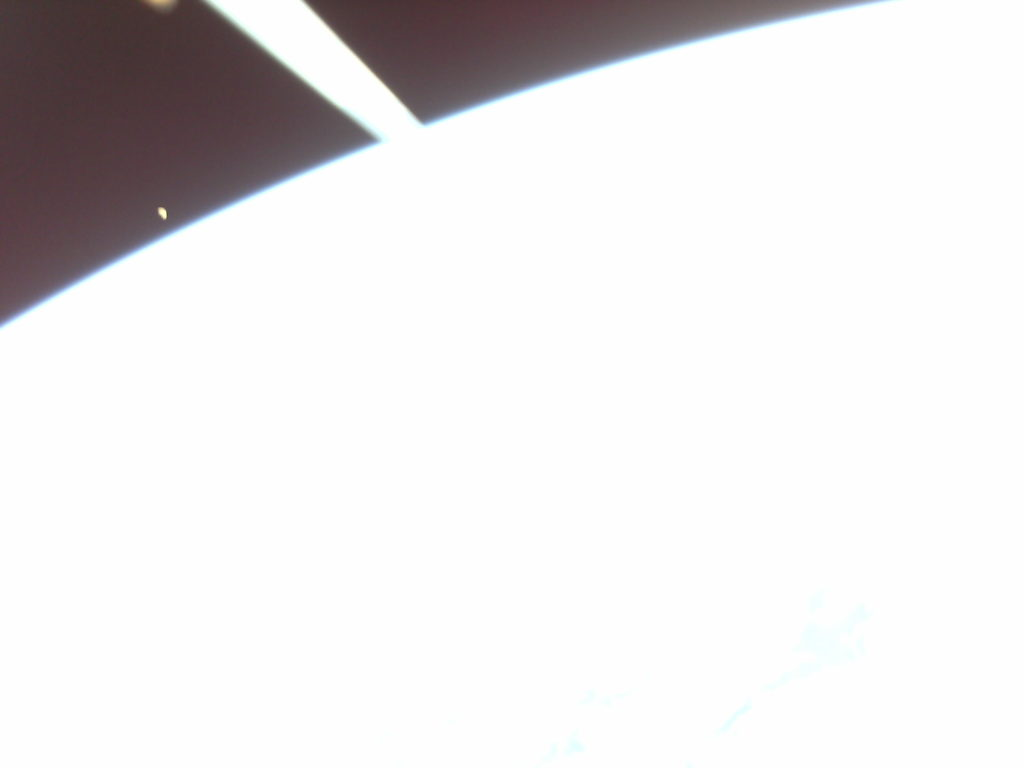
\includegraphics[width=9.5cm]{figures/stf-1-ex4.jpg}
        \end{center}
    \end{figure}

\end{frame}

\begin{frame}{Custom Projects: \href{http://stf1.com/}{\textcolor{cyan}{\underline{STF-1}}}}

    \begin{figure}[!ht]
        \begin{center}
            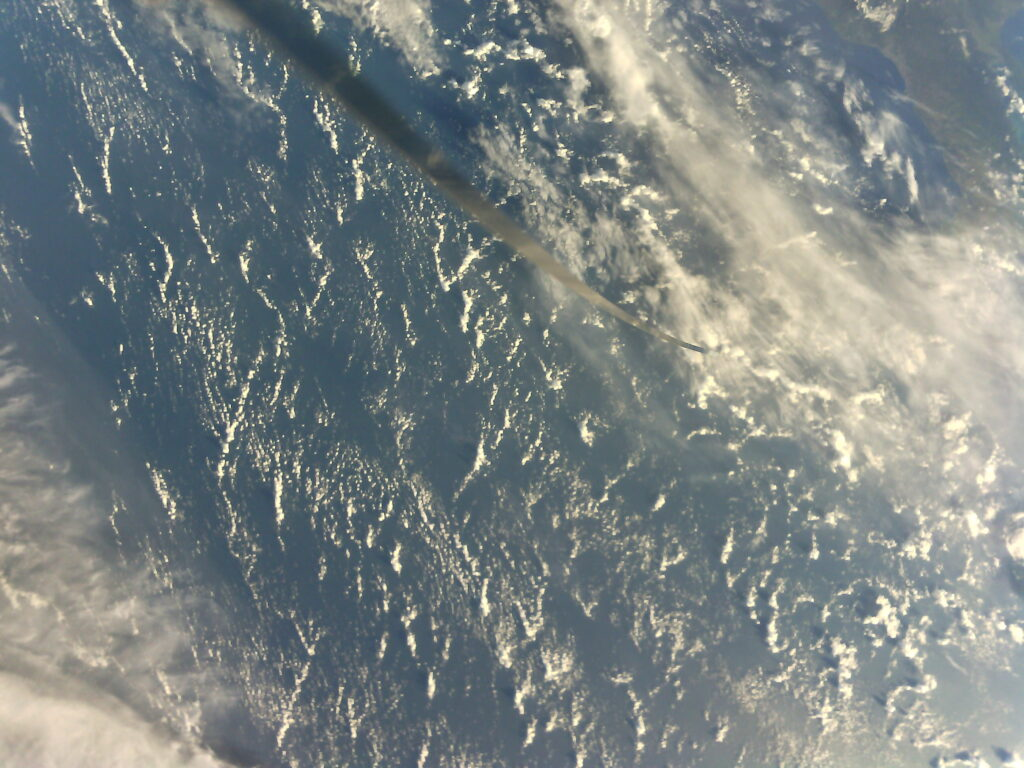
\includegraphics[width=9.5cm]{figures/stf-1-ex5.jpg}
        \end{center}
    \end{figure}

\end{frame}

\begin{frame}{Custom Projects: \href{http://stf1.com/}{\textcolor{cyan}{\underline{STF-1}}}}

    \begin{figure}[!ht]
        \begin{center}
            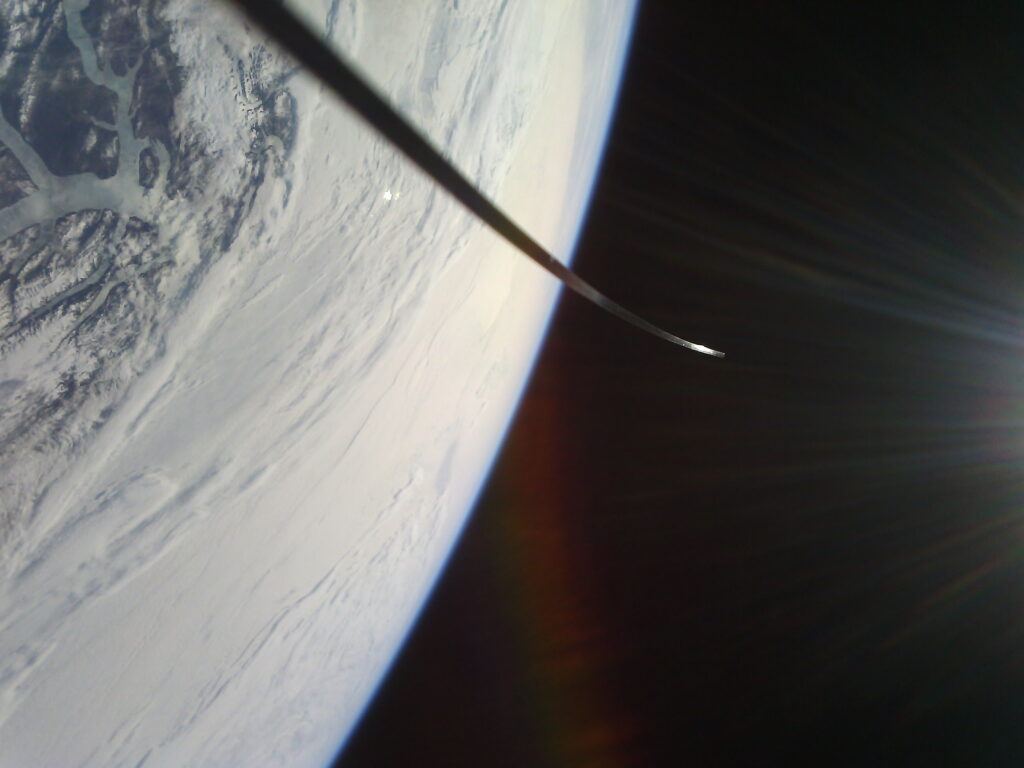
\includegraphics[width=9.5cm]{figures/stf-1-ex6.jpg}
        \end{center}
    \end{figure}

\end{frame}